\documentclass{article}
\usepackage{graphicx} % Required for inserting images
\usepackage[utf8]{inputenc}
\usepackage[greek,english]{babel}
\usepackage{amsmath}
\usepackage{tcolorbox} 
\usepackage{xcolor}
\usepackage{array}
\usepackage{enumitem}
\usepackage{multirow}
\usepackage{graphicx}
\usepackage{booktabs}

\title{Assignment in Numerical Analysis LaTeX}
\author{Full Name: Savvidis Theocharis 4555}
\date{ January 2024}

\begin{document}


\maketitle

\section{Fifth Exercise}
\subsection{Polynomial approximation}
For the Polynomial approximation the Lagrange polynomial was used.

\begin{tcolorbox}[colback=red!10, colframe=gray!80, width=\textwidth, sharp corners]
    \centering 
    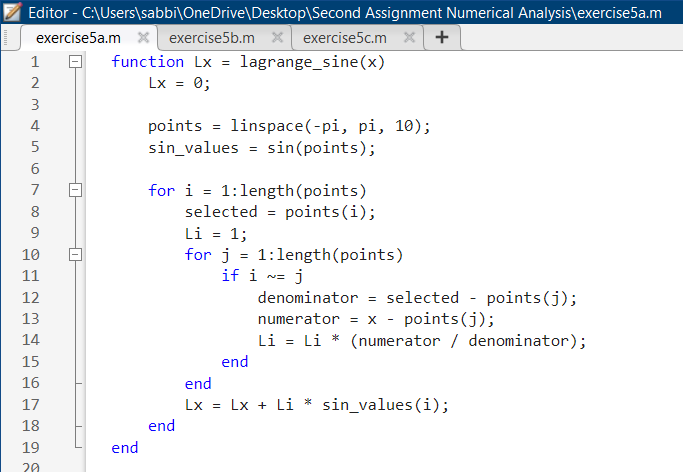
\includegraphics[width=0.5\textwidth,height=0.21\textheight]{Exercise5aCode.png} 

    \vspace{0.5cm}
    \small\textit{Note: The code was implemented without the assistance of a language model. }
\end{tcolorbox}

Testing 200 different values in the interval $ [-\pi,\pi]$ ,\textbf{ 7 digits of precision} are obtained.

\begin{tcolorbox}[colback=red!10, colframe=gray!80, width=\textwidth, sharp corners]
    \centering 
    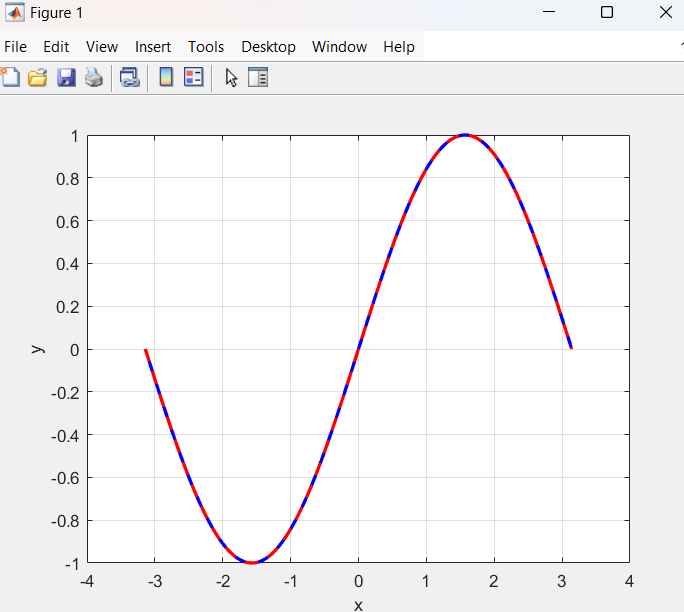
\includegraphics[width=0.5\textwidth,height=0.21\textheight]{Exercise5aPlot.png} 

    \vspace{0.5cm}
    \small\textit{Note: The plot displaying the curve created by 200 values using the Polynomial approximation alongside the plot of sine. }
\end{tcolorbox}
\subsection{Splines}
\begin{tcolorbox}[colback=red!10, colframe=gray!80, width=\textwidth, sharp corners]
    \centering 
    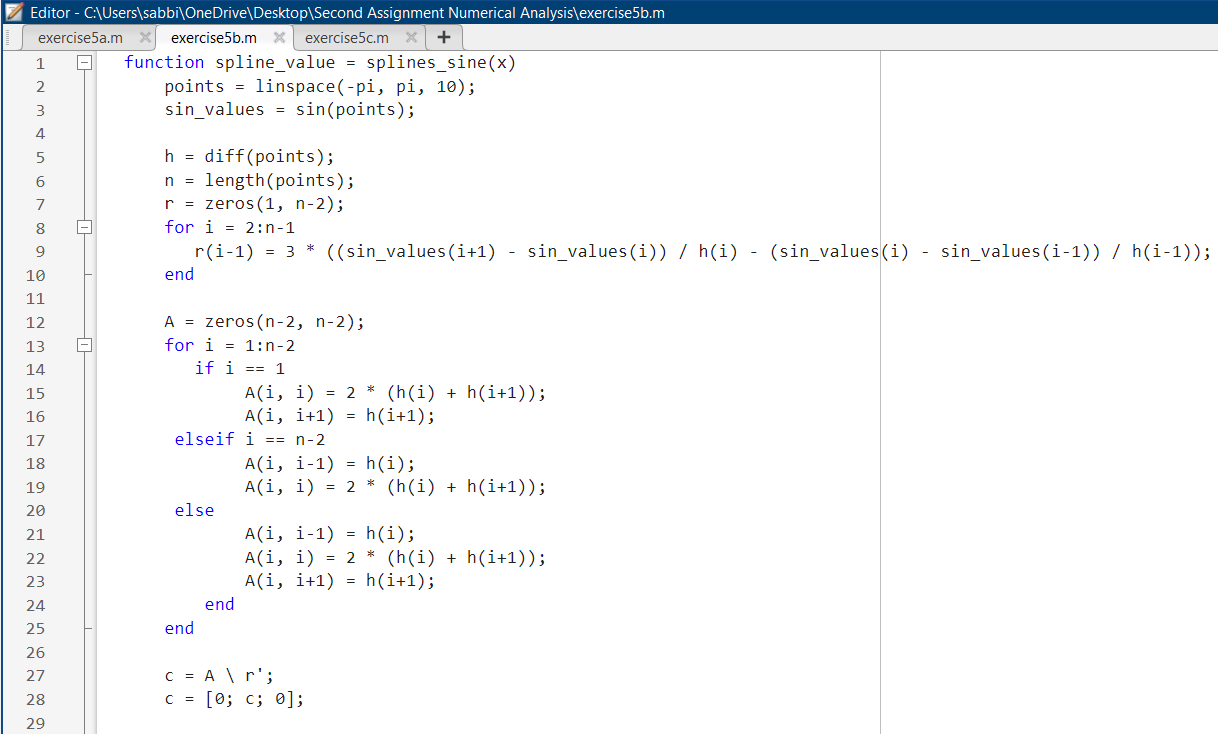
\includegraphics[width=0.6\textwidth,height=0.21\textheight]{Exercise5bCode.png} 
    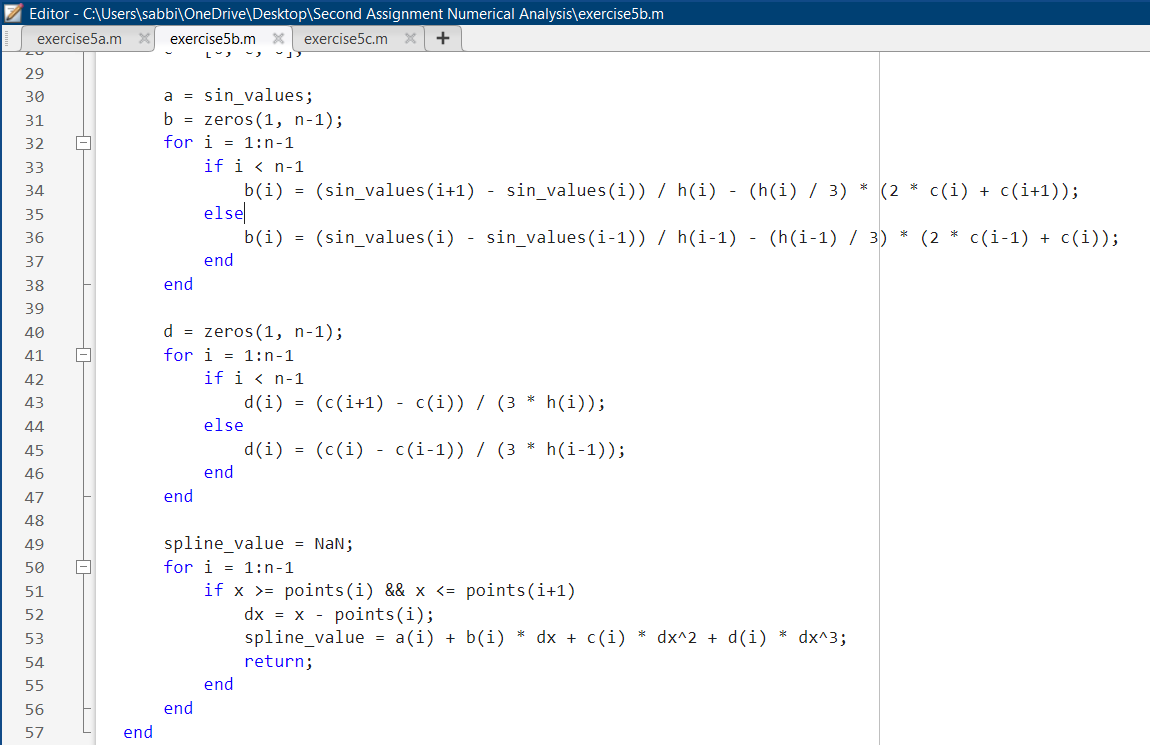
\includegraphics[width=0.6\textwidth,height=0.21\textheight]{Exercise5bCode2.png} 


    
    \vspace{0.5cm}
    \small\textit{Note: The code was implemented without the assistance of a language model. }
\end{tcolorbox}
 Testing 200 different values in the interval $ [-\pi,2.4]$ (approximation),\textbf{ 4 digits of precision} are obtained , while in the interval $ [2.4,\pi]$ the error is increasing as shown at the plot, losing precision digits continually.
  

\begin{tcolorbox}[colback=red!10, colframe=gray!80, width=\textwidth, sharp corners]
    \centering 
    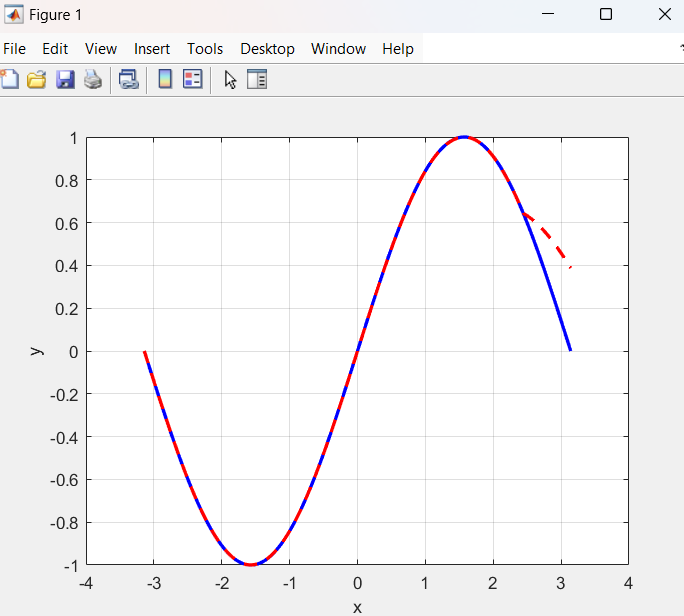
\includegraphics[width=0.5\textwidth,height=0.21\textheight]{Exercise5bPlot.png} 

    \vspace{0.5cm}
    \small\textit{Note: The plot displaying the curve created by 200 values using  Splines alongside the plot of sine. }
\end{tcolorbox}  
\subsection{Least Squares}
\begin{tcolorbox}[colback=red!10, colframe=gray!80, width=\textwidth, sharp corners]
    \centering 
    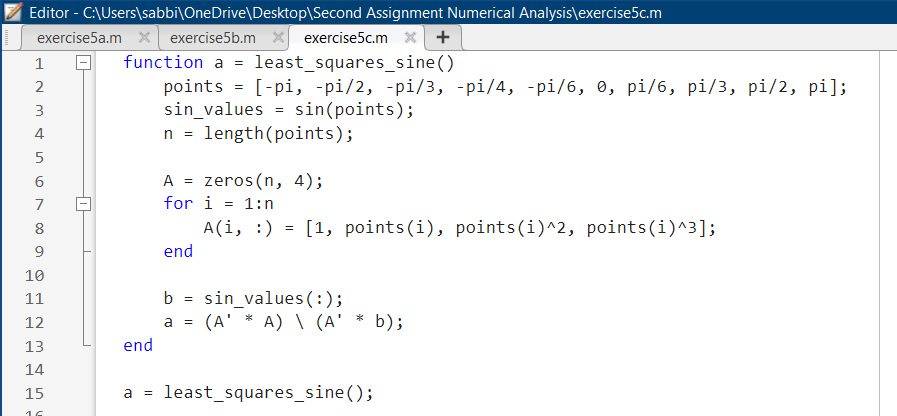
\includegraphics[width=0.6\textwidth,height=0.19\textheight]{Exercise5cCode.png} 

    
    \vspace{0.5cm}
    \small\textit{Note: For the implementation of the Least Squares method , a polynomial of degree 3 was used.}
\end{tcolorbox}

Testing 200 different values in the interval $ [-\pi,\pi]$ ,\textbf{ 1 digit of precision} is obtained.

\begin{tcolorbox}[colback=red!10, colframe=gray!80, width=\textwidth, sharp corners]
    \centering 
    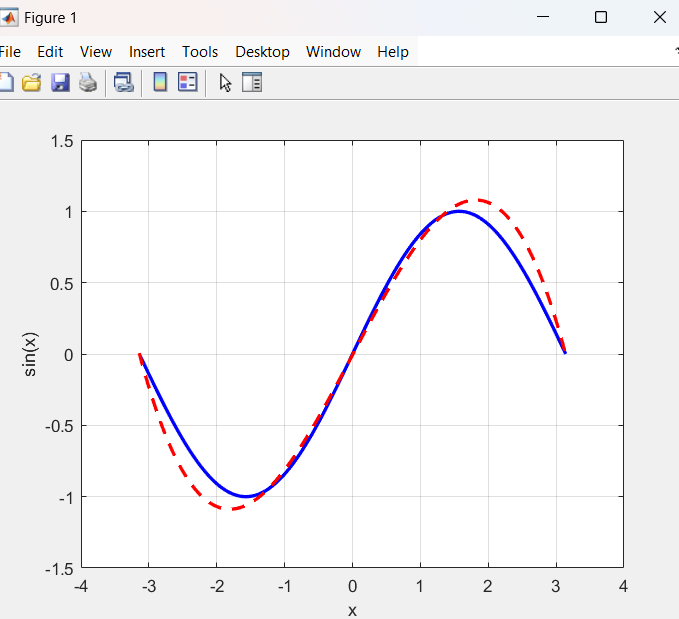
\includegraphics[width=0.6\textwidth,height=0.19\textheight]{Exercise5cPlot.png} 

    
    \vspace{0.5cm}
    \small\textit{Note: The plot displaying the curve created by 200 values using the Least squares alongside the plot of sine. }
\end{tcolorbox}
\subsection{Comparison}
Based on the specific implementations and the choices made (Lagrange polynomial , 3rd degree polynomial used in Least Squares)\textbf{ most precision is achieved using the Polynomial approximation} (the first method used) as 7 digits of precision are obtained in comparison with the 4 and 1 precision digits obtained by the following methods of Splines and Least squares correspondingly.

\section{Sixth Exercise}
\subsection{Simpson}
The implementation of the Simpson method for the sine function using 11 points between the interval $[0,\pi]$ leads to the \textbf{result 1.000003} ,thus the numerical \textbf{error }is  $1.000003-1=\textbf{0.000003}$ ,considering that \[
\int_{0}^{\frac{\pi}{2}} \sin(x) \, dx = 1
\] 
The \textbf{theoretical error} as calculated by the code below is \textbf{0.000008}.
\begin{tcolorbox}[colback=red!10, colframe=gray!80, width=\textwidth, sharp corners]
    \centering 
    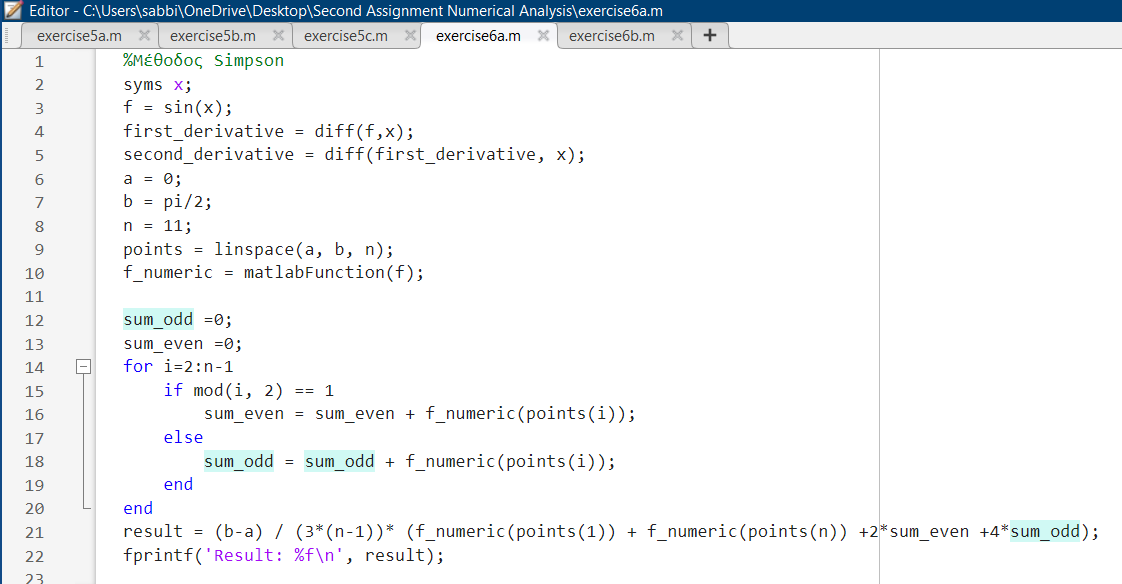
\includegraphics[width=0.75\textwidth,height=0.23\textheight]{Exercise6aCode.png} 

    \vspace{0.1cm}
    \small\textit{Note: Code implementing the Simpson method. }
\end{tcolorbox}

\begin{tcolorbox}[colback=red!10, colframe=gray!80, width=\textwidth, sharp corners]
    \centering 
    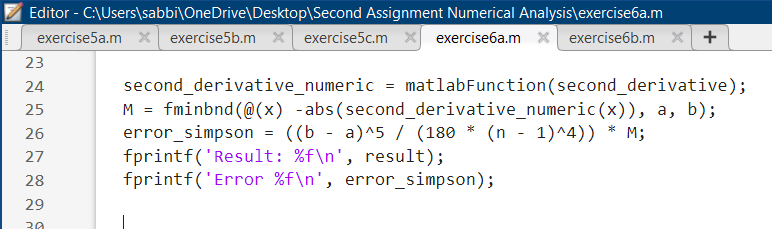
\includegraphics[width=0.8\textwidth,height=0.12\textheight]{Exercise6aError.png} 

    \vspace{0.1cm}
    \small\textit{Note: Code calculating the theoretical error of the Simpson method. }
\end{tcolorbox}

\subsection{Trapezoid Rule}

The implementation of the Trapezoid Rule for the sine function using 11 points between the interval $[0,\pi]$ leads to the \textbf{result 0.997943} ,thus the numerical \textbf{error }is  $1-0.997943 = \textbf{0.002057}$ ,considering that \[
\int_{0}^{\frac{\pi}{2}} \sin(x) \, dx = 1
\] 
The \textbf{theoretical error} as calculated by the code below is \textbf{0.005073}.



\begin{tcolorbox}[colback=red!10, colframe=gray!80, width=\textwidth, sharp corners]
    \centering 
    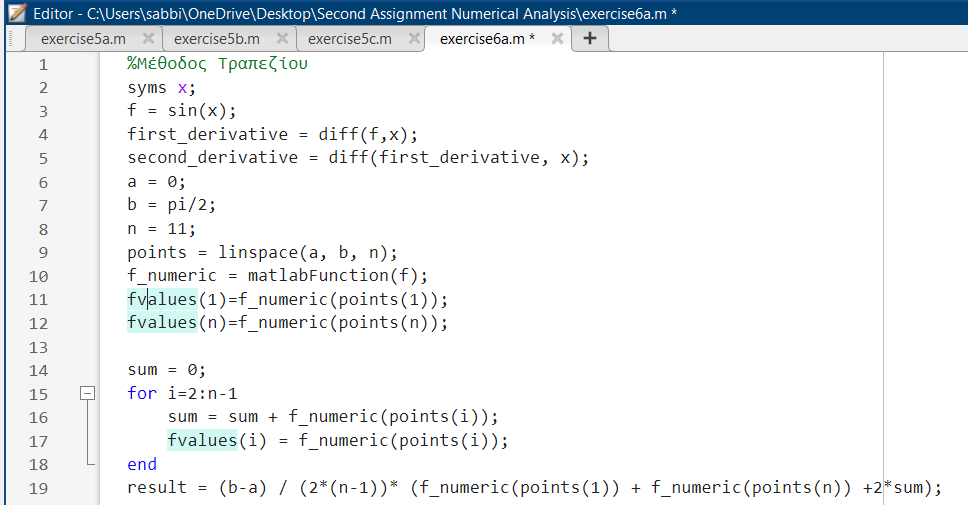
\includegraphics[width=0.7\textwidth,height=0.2\textheight]{Exercise6bCode.png} 

    \vspace{0.1cm}
    \small\textit{Note: Code implementing the Trapezoid Rule. }
\end{tcolorbox}

\begin{tcolorbox}[colback=red!10, colframe=gray!80, width=\textwidth, sharp corners]
    \centering 
    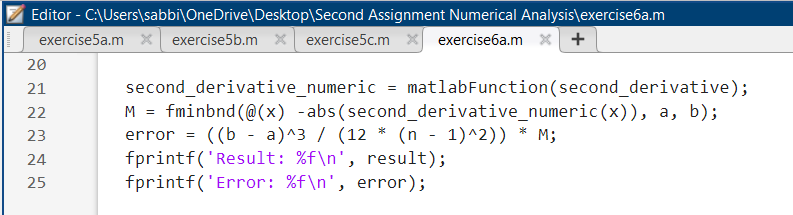
\includegraphics[width=0.8\textwidth,height=0.12\textheight]{Exercise6bError.png} 

    \vspace{0.1cm}
    \small\textit{Note: Code for calculating the theoretical error of the Trapezoid Rule. }
\end{tcolorbox}
\newpage
\vspace{5cm}
\section{Seventh Exercise}


\begin{itemize}
    \item \textbf{Conclusions and Quality Comparison}
    
    The two stocks used from the Athens Stock Market were\textbf{ LAMDA} and      \textbf{KPI-KPI}.As a base \textbf{date} the \textbf{5/7/2024} was used and predictions were made for the next six days that the stock market was open (8/7/2024 - 15/7/2024).

    It is evident that the \textbf{predictions} for the dates after the known prices are more accurate using the lower degree polynomial (the second degree) as it is the less volatile than the other two (third and fourth degree polynomials).
    \textbf{As the distance from the known prices increases, predictions made using a higher degree polynomials are becoming more and more extreme} ,thus usually diverge significantly from the actual values as they adapt more efficiently to the known points-prices.

    
    As for the \textbf{approximations} \textbf{for the known prices} using both the second ,third and fourth degree polynomials are close to the real values. It can be observed that \textbf{as the degree of the polynomial increases , the approximations made are closer to the real values.}

    
    

\end{itemize}

\newpage
\subsection{KPI-KPI Stock}

\begin{itemize}
    \item \textbf{Using a second degree polynomial }
\begin{tcolorbox}[colback=red!10, colframe=gray!80, width=\textwidth, sharp corners]
    \centering 
    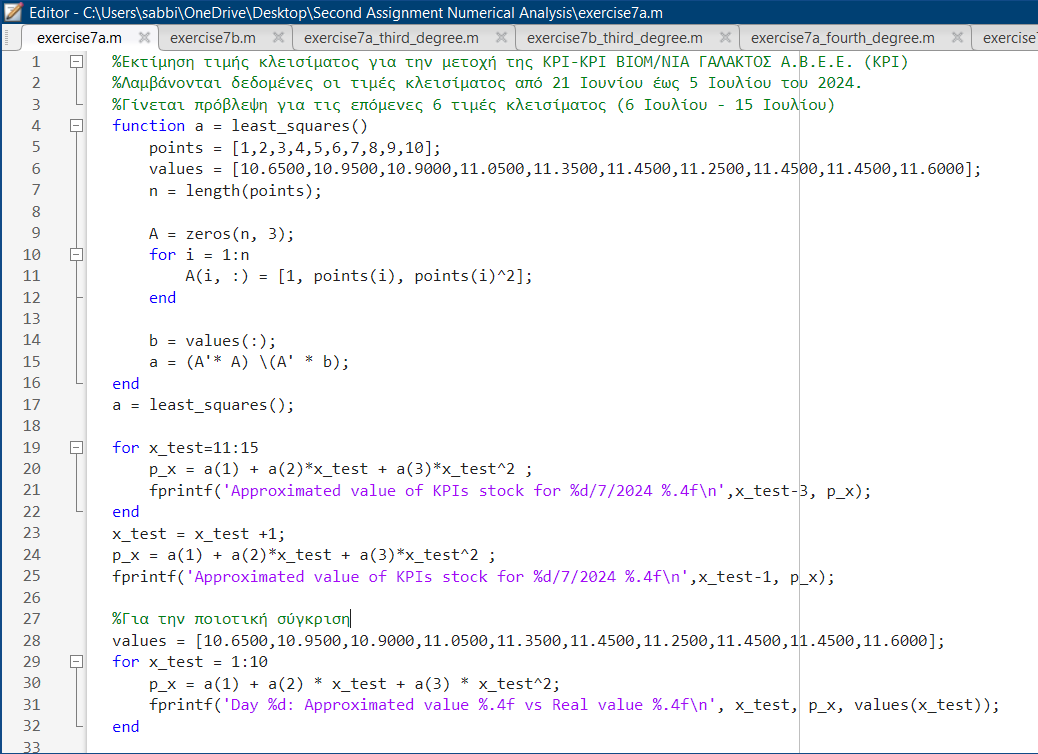
\includegraphics[width=0.8\textwidth,height=0.38\textheight]{Exercise7aSecond.png} 

    \vspace{0.1cm}
    \small\textit{Note: Code implementing the Least Squares method with a \textbf{second degree polynomial} using 10 known closing prices of KPI-KPI's stock. }
\end{tcolorbox}


As it is displayed below, the \textbf{predictions} for the day after the known closing prices as well as the other 5 consecutive closing price predictions for KPI-KPI's stock for the dates after 5/7/2024 with an open stock market are:
\begin{center}
    \begin{tabular}{|c|c|}
        \hline
        \textbf{Date} & \textbf{Predicted Value of KPI's Stock} \\
        \hline
        8/7/2024 & 11.5475 \\
        9/7/2024 & 11.5437 \\
        10/7/2024 & 11.5236 \\
        11/7/2024 & 11.4873 \\
        12/7/2024 & 11.4346 \\
        15/7/2024 & 11.3657 \\
        \hline
    \end{tabular}
\end{center}

Also for the \textbf{already known} values the \textbf{approximations} using the second degree polynomial are the following:
\begin{table}[h!]
    \centering
    \begin{tabular}{@{}ccc@{}}
        \toprule
        \textbf{Day} & \textbf{Approximated Value} & \textbf{Real Value} \\ \midrule
        1 & 10.6895 & 10.6500 \\
        2 & 10.8486 & 10.9500 \\
        3 & 10.9914 & 10.9000 \\
        4 & 11.1180 & 11.0500 \\
        5 & 11.2282 & 11.3500 \\
        6 & 11.3221 & 11.4500 \\
        7 & 11.3998 & 11.2500 \\
        8 & 11.4611 & 11.4500 \\
        9 & 11.5062 & 11.4500 \\
        10 & 11.5350 & 11.6000 \\
        \bottomrule
    \end{tabular}

    
\end{table}
\newpage
    \item \textbf{Using a third degree polynomial}
    \begin{tcolorbox}[colback=red!10, colframe=gray!80, width=\textwidth, sharp corners]
    \centering 
    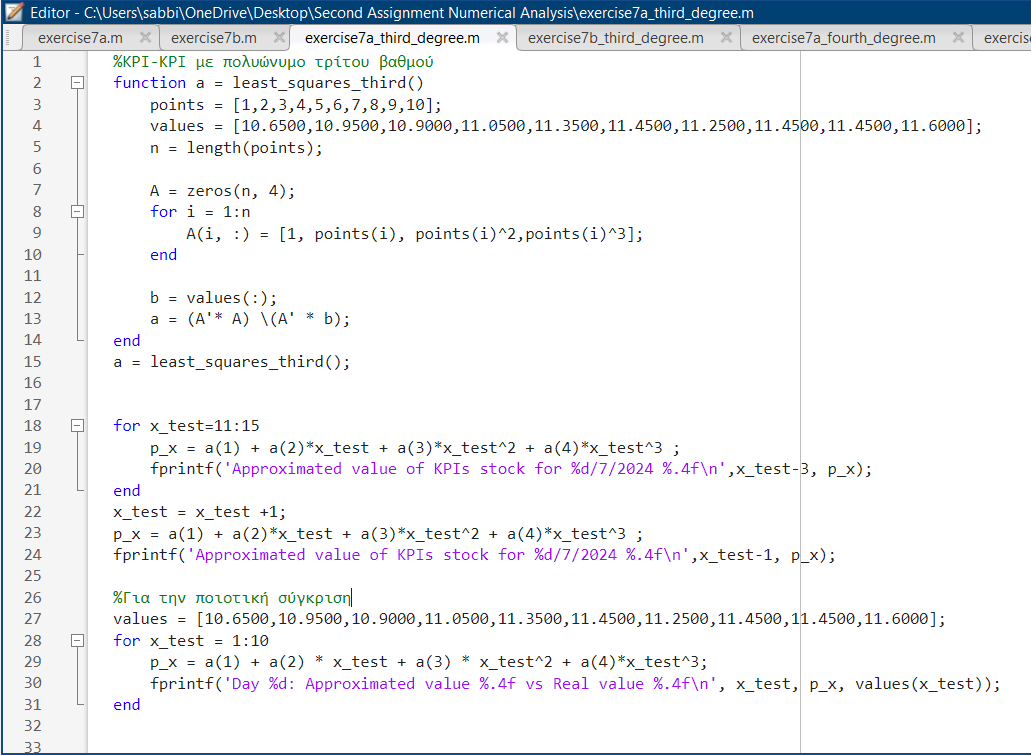
\includegraphics[width=0.8\textwidth,height=0.38\textheight]{Exercise7aThird.png} 

    \vspace{0.1cm}
    \small\textit{Note: Code implementing the Least Squares method with a \textbf{third degree polynomial} using 10 known closing prices of KPI-KPI's stock. }
\end{tcolorbox}


As it is displayed below, the \textbf{predictions} for the day after the known closing prices as well as the other 5 consecutive closing price predictions for KPI-KPI's stock for the dates after 5/7/2024 with an open stock market are:
\begin{center}
    \begin{tabular}{|c|c|}
        \hline
        \textbf{Date} & \textbf{Predicted Value of KPI's Stock} \\
        \hline
        8/7/2024 & 11.6517 \\
        9/7/2024 & 11.7615 \\
        10/7/2024 & 11.9024 \\
        11/7/2024 & 12.0817 \\
        12/7/2024 & 12.3066 \\
        15/7/2024 & 12.5844 \\
        \hline
    \end{tabular}
\end{center}

Also for the \textbf{already known} values the \textbf{approximations} using the third degree polynomial are the following:
\begin{center}
    

    \begin{tabular}{@{}ccc@{}}
        \toprule
        \textbf{Day} & \textbf{Approximated Value} & \textbf{Real Value} \\ \midrule
        1 & 10.6590 & 10.6500 \\
        2 & 10.8588 & 10.9500 \\
        3 & 11.0169 & 10.9000 \\
        4 & 11.1405 & 11.0500 \\
        5 & 11.2369 & 11.3500 \\
        6 & 11.3134 & 11.4500 \\
        7 & 11.3772 & 11.2500 \\
        8 & 11.4356 & 11.4500 \\
        9 & 11.4960 & 11.4500 \\
        10 & 11.5656 & 11.6000 \\
        \bottomrule
    \end{tabular}

    \end{center}
    \item \textbf{Using a fourth degree polynomial}
    \begin{tcolorbox}[colback=red!10, colframe=gray!80, width=\textwidth, sharp corners]
    \centering 
    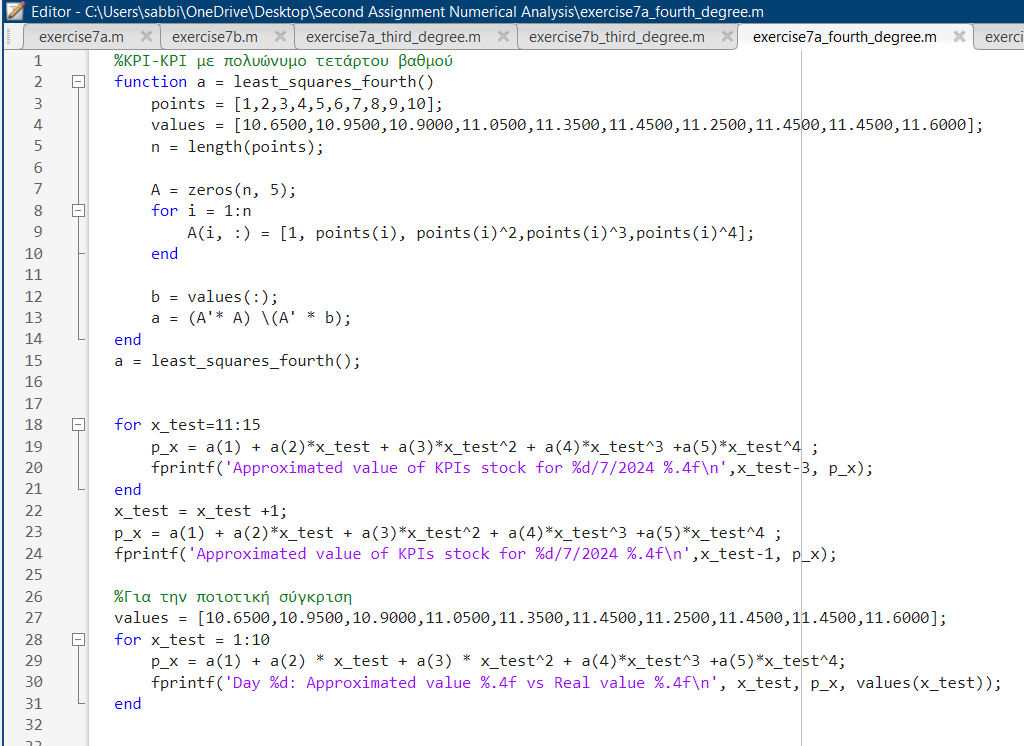
\includegraphics[width=0.8\textwidth,height=0.38\textheight]{Exercise7aFourth.png} 

    \vspace{0.1cm}
    \small\textit{Note: Code implementing the Least Squares method with a \textbf{fourth degree polynomial} using 10 known closing prices of KPI-KPI's stock. }
\end{tcolorbox}


As it is displayed below, the \textbf{predictions} for the day after the known closing prices as well as the other 5 consecutive closing price predictions for KPI-KPI's stock for the dates after 5/7/2024 with an open stock market are:

\begin{center}
    \begin{tabular}{|c|c|}
        \hline
        \textbf{Date} & \textbf{Predicted Value of KPI's Stock} \\
        \hline
        8/7/2024 & 11.9042 \\
        9/7/2024 & 12.4731 \\
        10/7/2024 & 13.4174 \\
        11/7/2024 & 14.8680 \\
        12/7/2024 & 16.9734 \\
        15/7/2024 & 19.8998 \\
        \hline
    \end{tabular}
\end{center}

Also for the \textbf{already known} values the \textbf{approximations} using the fourth degree polynomial are the following:
\begin{center}
    
    \begin{tabular}{@{}ccc@{}}
        \toprule
        \textbf{Day} & \textbf{Approximated Value} & \textbf{Real Value} \\ \midrule
        1 & 10.6907 & 10.6500 \\
        2 & 10.8200 & 10.9500 \\
        3 & 10.9869 & 10.9000 \\
        4 & 11.1458 & 11.0500 \\
        5 & 11.2687 & 11.3500 \\
        6 & 11.3452 & 11.4500 \\
        7 & 11.3825 & 11.2500 \\
        8 & 11.4056 & 11.4500 \\
        9 & 11.4572 & 11.4500 \\
        10 & 11.5974 & 11.6000 \\
        \bottomrule
    \end{tabular}

    \end{center}
\end{itemize}
\newpage
\subsection{LAMDA Stock}

\begin{itemize}
    \item \textbf{Using a second degree polynomial }

\begin{tcolorbox}[colback=red!10, colframe=gray!80, width=\textwidth, sharp corners]
    \centering 
    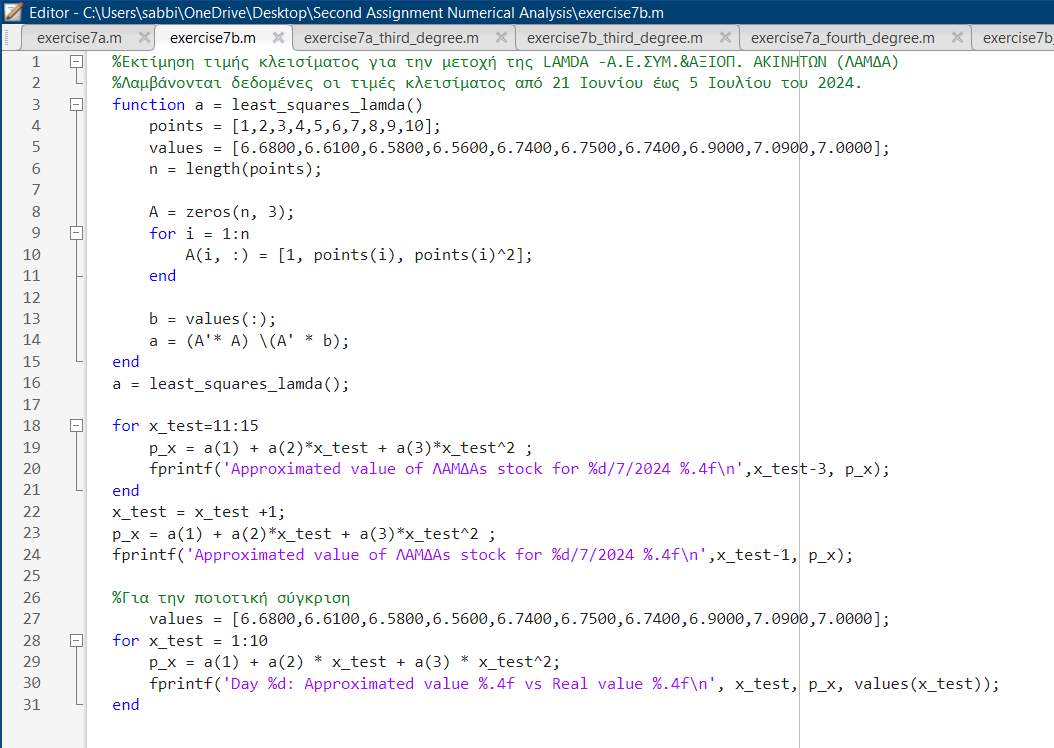
\includegraphics[width=0.8\textwidth,height=0.38\textheight]{Exercise7bSecond.png} 

    \vspace{0.1cm}
    \small\textit{Note: Code implementing the Least Squares method with a \textbf{second degree polynomial} using 10 known closing prices of LAMDA's stock. }
\end{tcolorbox}

    As it is displayed below, the \textbf{predictions} for the day after the known closing prices as well as the other 5 consecutive closing price predictions for LAMDA's stock for the dates after 5/7/2024 with an open stock market are:
    \begin{center}
    \begin{tabular}{|c|c|}
        \hline
        \textbf{Date} & \textbf{Predicted Value of LAMDA's Stock} \\
        \hline
        8/7/2024 & 7.2230 \\
        9/7/2024 & 7.3711 \\
        10/7/2024 & 7.5355 \\
        11/7/2024 & 7.7160 \\
        12/7/2024 & 7.9128 \\
        15/7/2024 & 8.1257 \\
        \hline
    \end{tabular}
\end{center}

Also for the \textbf{already known} values the \textbf{approximations} using the second degree polynomial are the following:
\begin{center}
    
    
    \centering
    \begin{tabular}{@{}ccc@{}}
        \toprule
        \textbf{Day} & \textbf{Approximated Value} & \textbf{Real Value} \\ \midrule
        1 & 6.6335 & 6.6800 \\
        2 & 6.6195 & 6.6100 \\
        3 & 6.6217 & 6.5800 \\
        4 & 6.6401 & 6.5600 \\
        5 & 6.6747 & 6.7400 \\
        6 & 6.7256 & 6.7500 \\
        7 & 6.7926 & 6.7400 \\
        8 & 6.8759 & 6.9000 \\
        9 & 6.9754 & 7.0900 \\
        10 & 7.0911 & 7.0000 \\ \bottomrule
    \end{tabular}
    \end{center}
    

  \item \textbf{Using a third degree polynomial}
  \begin{tcolorbox}[colback=red!10, colframe=gray!80, width=\textwidth, sharp corners]
    \centering 
    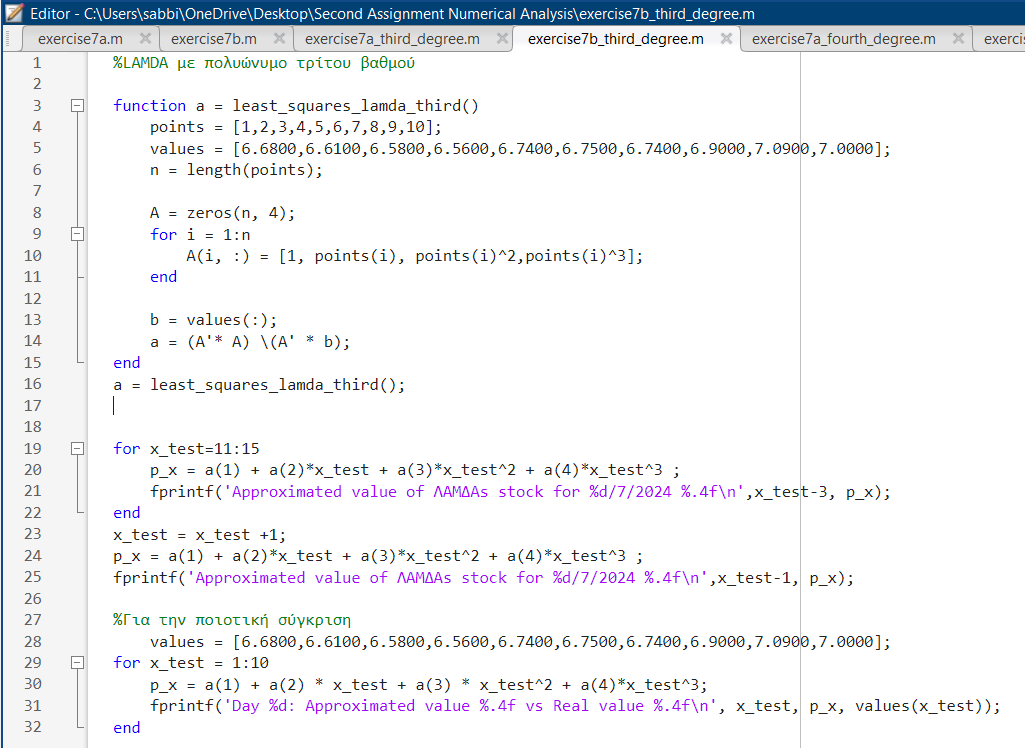
\includegraphics[width=0.8\textwidth,height=0.38\textheight]{Exercise7bThird.png} 

    \vspace{0.1cm}
    \small\textit{Note: Code implementing the Least Squares method with a \textbf{third degree polynomial} using 10 known closing prices of LAMDA's stock. }
\end{tcolorbox}

    As it is displayed below, the \textbf{predictions} for the day after the known closing prices as well as the other 5 consecutive closing price predictions for LAMDA's stock for the dates after 5/7/2024 with an open stock market are:
    \begin{center}
    \begin{tabular}{|c|c|}
        \hline
        \textbf{Date} & \textbf{Predicted Value of LAMDA's Stock} \\
        \hline
        8/7/2024 & 7.0533 \\
        9/7/2024 & 7.0164 \\
        10/7/2024 & 6.9185 \\
        11/7/2024 & 6.7478 \\
        12/7/2024 & 6.4925 \\
        15/7/2024 & 6.1407 \\
        \hline
    \end{tabular}
\end{center}

Also for the \textbf{already known} values the \textbf{approximations} using the third degree polynomial are the following:
\begin{center}
    
    
    \centering
     \begin{tabular}{@{}ccc@{}}
        \toprule
        \textbf{Day} & \textbf{Approximated Value} & \textbf{Real Value} \\ \midrule
        1 & 6.6833 & 6.6800 \\
        2 & 6.6028 & 6.6100 \\
        3 & 6.5801 & 6.5800 \\
        4 & 6.6033 & 6.5600 \\
        5 & 6.6605 & 6.7400 \\
        6 & 6.7398 & 6.7500 \\
        7 & 6.8294 & 6.7400 \\
        8 & 6.9174 & 6.9000 \\
        9 & 6.9920 & 7.0900 \\
        10 & 7.0413 & 7.0000 \\ \bottomrule
    \end{tabular}
    \end{center}
\item \textbf{Using a fourth degree polynomial}
\begin{tcolorbox}[colback=red!10, colframe=gray!80, width=\textwidth, sharp corners]
    \centering 
    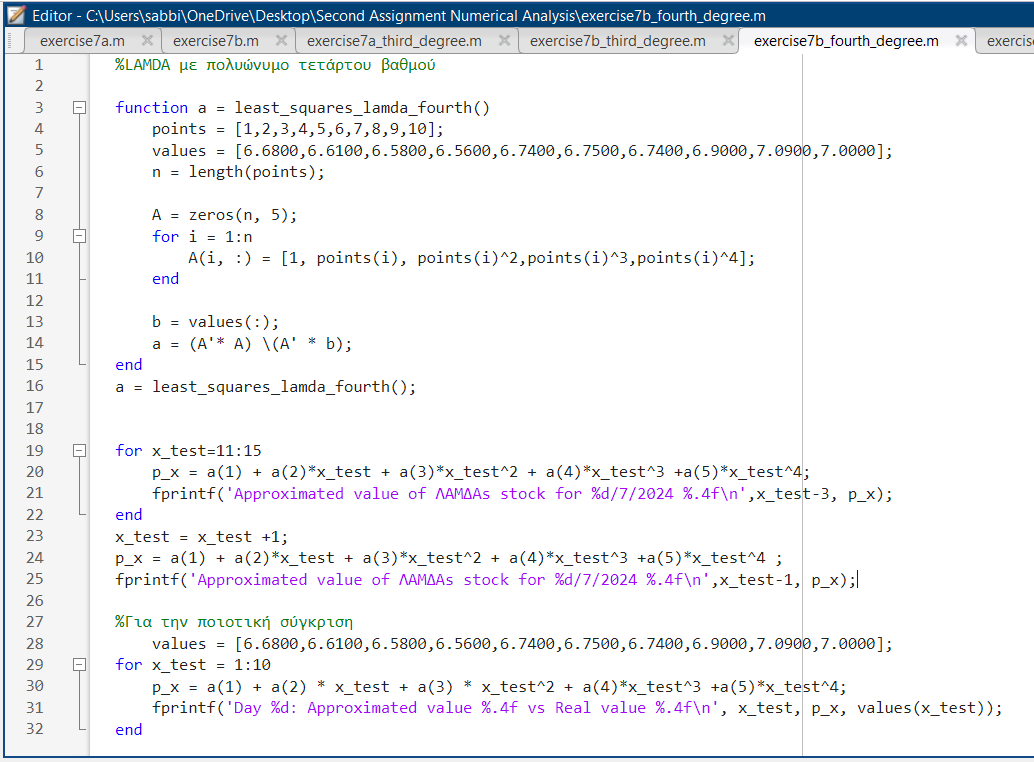
\includegraphics[width=0.8\textwidth,height=0.38\textheight]{Exercise7bFourth.png} 

    \vspace{0.1cm}
    \small\textit{Note: Code implementing the Least Squares method with a \textbf{fourth degree polynomial} using 10 known closing prices of LAMDA's stock. }
\end{tcolorbox}

    As it is displayed below, the \textbf{predictions} for the day after the known closing prices as well as the other 5 consecutive closing price predictions for LAMDA's stock for the dates after 5/7/2024 with an open stock market are:
    \begin{center}
    \begin{tabular}{|c|c|}
        \hline
        \textbf{Date} & \textbf{Predicted Value of LAMDA's Stock} \\
        \hline
        8/7/2024 & 6.9733 \\
        9/7/2024 & 6.7909 \\
        10/7/2024 & 6.4385 \\
        11/7/2024 & 5.8650 \\
        12/7/2024 & 5.0139 \\
        15/7/2024 & 3.8230 \\
        \hline
    \end{tabular}
\end{center}


Also for the \textbf{already known} values the \textbf{approximations} using the fourth degree polynomial are the following:
\begin{center}
    
    
    \centering
    \begin{tabular}{@{}ccc@{}}
        \toprule
        \textbf{Day} & \textbf{Approximated Value} & \textbf{Real Value} \\ \midrule
        1 & 6.6732 & 6.6800 \\
        2 & 6.6152 & 6.6100 \\
        3 & 6.5897 & 6.5800 \\
        4 & 6.6016 & 6.5600 \\
        5 & 6.6504 & 6.7400 \\
        6 & 6.7297 & 6.7500 \\
        7 & 6.8277 & 6.7400 \\
        8 & 6.9269 & 6.9000 \\
        9 & 7.0043 & 7.0900 \\
        10 & 7.0312 & 7.0000 \\ \bottomrule
    \end{tabular}
    \end{center}
\end{itemize}
    
   





\end{document}


